% !TEX root = ../master-thesis.tex


\begin{figure}
    \centering
    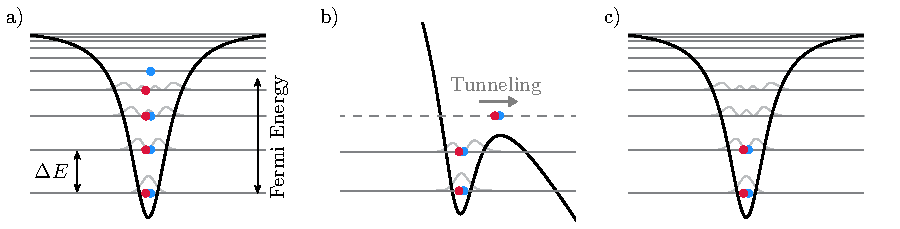
\includegraphics{fig-ai/preparation.pdf}
    \caption{
        \textbf{Deterministic preparation via spilling.}
        (a) Fermionic atoms are initially loaded into a tightly confined optical tweezer, forming a Fermi sea occupying the approximately 1D harmonic oscillator levels up to the Fermi energy. 
        (b) A magnetic field gradient tilts the potential, and the trap depth is lowered such that atoms above a defined spill level tunnel out. 
        (c) This procedure leaves a well-defined number of atoms in the lowest energy states, with a preparation fidelity of approximately 95\%. 
        Blue and red dots denote atoms in different spin states; gray curves indicate the bound-state wavefunctions.
    }
    \label{fig:preparation}
\end{figure}


Quantum simulation of strongly correlated many-body systems requires precise control over initial quantum states to access regimes beyond thermal equilibrium and investigate specific quantum phenomena. The ability to prepare designer initial states with single-site and single-spin resolution has become essential for studying complex quantum phases, far-from-equilibrium dynamics, and engineered many-body Hamiltonians. Beyond fundamental many-body physics, deterministic state preparation is crucial for quantum chemistry simulations~\cite{gkritsis_simulating_2025}, and for broader fermionic quantum computing applications~\cite{gonzalez-cuadra_fermionic_2023}.
% This capability is particularly important for distinguishing between different dynamical regimes, such as many-body localization (MBL) and Anderson localization, where the initial state configuration directly influences the observable signatures and relaxation dynamics.

Traditional approaches for loading atoms into optical lattices rely on transferring atomic clouds from magneto-optical traps (MOTs) or optical dipole traps (ODTs) into the periodic potential created by interfering laser beams. While these methods have enabled significant progress in quantum simulation, they face fundamental limitations in state preparation flexibility. The primary constraint arises from the lack of sufficiently different spin-dependent potentials that would enable site-selective manipulation of internal atomic degrees of freedom. Although spatial light modulators (SLMs) and digital micromirror devices (DMDs) can create programmable optical potentials for compensating harmonic confinement and achieving uniform filling~\cite{mazurenko_cold-atom_2017}, the construction of arbitrary spin-resolved configurations remains challenging with conventional lattice-loading techniques.

Optical tweezers have also been employed to enhance conventional thermal loading approaches through site-resolved addressing. Notable implementations include using individual tweezers to locally increase the potential depth during lattice loading, thereby creating controlled defects in otherwise uniformly filled systems~\cite{koepsell_imaging_2019}. Such hybrid approaches have enabled studies of antiferromagnetic order with engineered impurities.
% , starting from near-Mott insulating conditions at temperatures around $0.45t$ with interaction strength $U/t = 14$. 
However, these methods still rely fundamentally on thermal equilibration and are limited in their ability to construct arbitrary initial configurations.

The emergence of optical tweezer arrays has provided a transformative solution to these state preparation challenges through deterministic, bottom-up assembly of many-body quantum systems~\cite{serwane_deterministic_2011}. Unlike traditional loading approaches that rely on statistical distributions, tweezer-based methods enable constructive control over both spatial and internal degrees of freedom. Early demonstrations showed the feasibility of deterministic few-body preparation in one-dimensional systems, with achieved fidelities of approximately 95\% for doublon preparation~\cite{holten_pauli_2022,spar_realization_2022}. Recent advances have extended these capabilities to one-dimensional tweeyer arrays~\cite{stuart_single-atom_2018,gyger_continuous_2024,spar_realization_2022}.

The core principle underlying tweezer-based state preparation involves the spilling technique, which exploits the quantized energy levels of fermions in tightly confined optical potentials. By adiabatically reducing the trap depth while applying magnetic field gradients, atoms occupying higher energy levels become unbound and escape, while those in lower levels remain trapped. The differential magnetic moments of hyperfine ground states enable spin-selective spilling: at specific magnetic field strengths, only one spin component experiences significant forces from applied gradients, allowing deterministic preparation of sites containing empty, single spin-up, single spin-down, or spin-paired configurations.

As part of this work, a tweezer array system was developed based on crossed acousto-optic deflectors (AODs), enabling spin-selective two-dimensional individual site control. The system aims deterministic preparation of arbitrary spin- and site-resolved occupation patterns through a sequence of global and spin-selective spilling operations. Current preparation fidelities reach 81\% for doublon preparation, with identified improvements in magnetic field stabilization expected to approach the 95\% benchmarks demonstrated in other laboratories~\cite{holten_pauli_2022,serwane_deterministic_2011,spar_realization_2022}.

To the best of our knowledge, arbitrary spin-selective state preparation in two-dimensional fermionic systems has not been previously demonstrated. 
% This capability represents a significant advancement for investigating dynamics of different Hamiltonians and implementing quantum chemistry simulations~\cite{gkritsis_simulating_2025}. 
The achievement of programmable spin-selective filling constitutes one of the central results of this work. Despite currently modest fidelities, the proposed methods appear promising for future developments in quantum simulation of strongly correlated fermions.

The integration of deterministic state preparation with the spin-resolved imaging capabilities described in Section~\ref{sec:imaging} provides the experimental tools necessary for systematic investigation of quantum many-body dynamics. The ability to prepare specific initial configurations and measure their subsequent evolution with single-site, single-shot resolution enables direct study of phenomena such as quantum thermalization and localization. 
% As demonstrated through numerical simulations in Section~\ref{sec:fhmodel}, the distinction between MBL and Anderson localisation dynamical regimes depends on both the initial state preparation and the measurement of local observables including density profiles, magnetization patterns, and correlation functions.

This chapter presents the design, implementation, and characterization of the complete tweezer array system. Section~\ref{subsec:aodconcept} describes the optical setup and acousto-optic deflector control systems. Section~\ref{subsec:control} details the calibration procedures for achieving uniform tweezer arrays and precise depth control. Section~\ref{subsec:state-prepation} presents the spilling protocols for deterministic few-body preparation. Section~\ref{subsec:spin-selective-spilling} introduces the spin-selective manipulation techniques enabling arbitrary spin-resolved configurations. Section~\ref{subsec:arbitrary-occupation-loading} demonstrates the complete sequence for preparing complex many-body initial states. The developed platform provides a foundation for future quantum simulation experiments investigating strongly correlated fermions in engineered two-dimensional systems.